% ВКР: Исследование механизмов повышения надёжности сервиса в федерации
% Kubernetes-кластеров. Сборка: make thesis (из корня репозитория).
% Красным [TODO: ...] помечены места, которые нужно дописать вручную.
\documentclass[14pt,a4paper]{extreport}

\usepackage{cmap}
\usepackage[T2A]{fontenc}
\usepackage[utf8]{inputenc}
\usepackage[english,russian]{babel}
\usepackage[left=30mm,right=15mm,top=20mm,bottom=20mm]{geometry}
\usepackage{setspace}
\onehalfspacing
\usepackage{indentfirst}
\usepackage{amsmath,amssymb}
\usepackage{graphicx}
\graphicspath{{../../../analysis/}{figures/}}
\usepackage{booktabs,tabularx,array}
\usepackage{enumitem}
\setlist{nosep,leftmargin=*,labelindent=\parindent}
\usepackage{caption}
\captionsetup{labelsep=endash,font=small}
\usepackage{xcolor}
\usepackage{tikz}
\usepackage{float}
\usetikzlibrary{arrows.meta,positioning,fit,backgrounds,calc}
\usepackage{titlesec}
\usepackage{makecell}
\usepackage{tocloft}
\renewcommand{\cfttoctitlefont}{\hfill\normalfont\large\bfseries}
\renewcommand{\cftaftertoctitle}{\hspace*{\fill}}
\usepackage{url}
\usepackage[hidelinks]{hyperref}

% Заголовки: «Глава 1. Название», разделы «1.1. Название».
\titleformat{\chapter}[block]{\normalfont\large\bfseries\centering}{Глава \thechapter.}{0.5em}{}
\titlespacing*{\chapter}{0pt}{-20pt}{14pt}
\titleformat{\section}{\normalfont\normalsize\bfseries}{\thesection.}{0.5em}{}
\titleformat{\subsection}{\normalfont\normalsize\bfseries}{\thesubsection.}{0.5em}{}

% Оглавление: «Глава 1. ...» и точки до номера страницы.
\renewcommand{\cftchappresnum}{Глава }
\renewcommand{\cftchapaftersnum}{.}
\setlength{\cftchapnumwidth}{5.2em}
\renewcommand{\cftchapleader}{\cftdotfill{\cftdotsep}}
\renewcommand{\cftchapfont}{\normalfont}
\renewcommand{\cftchappagefont}{\normalfont}
\addto\captionsrussian{%
  \renewcommand{\contentsname}{Содержание}%
  \renewcommand{\bibname}{Список литературы}%
}

% Раздел без номера, но в оглавлении: Введение, Постановка задачи и т. д.
\newcommand{\unnumchapter}[1]{\chapter*{#1}\addcontentsline{toc}{chapter}{#1}}
\newcommand{\todo}[1]{{\color{red}[\textbf{TODO:} #1]}}

\begin{document}

% Титульный лист по образцу ВКР кафедры; английский вариант добавить по запросу.
\begin{titlepage}
\begin{center}
\singlespacing
Санкт-Петербургский государственный университет

\vspace{25mm}
\textbf{ТРОФИМОВ Иван Александрович}

\vspace{8mm}
\textbf{Выпускная квалификационная работа}

\vspace{4mm}
{\large\bfseries «Разработка системы управления размещением нагрузки
в федерации Kubernetes-кластеров с учётом метрик надёжности»\par}

\vspace{12mm}
\begin{flushleft}
Уровень образования: бакалавриат\\
Направление 02.03.02 «Фундаментальная информатика и информационные технологии»\\
Основная образовательная программа \todo{код} «Большие данные и распределённая цифровая платформа»
\end{flushleft}

\vfill
\begin{flushright}
\begin{minipage}{0.55\textwidth}
Научный руководитель:\\
кандидат физ.-мат. наук, доцент\\
Корхов Владимир Владиславович

\vspace{6mm}
Рецензент:\\
\todo{должность, степень, ФИО}
\end{minipage}
\end{flushright}

\vfill
Санкт-Петербург\\
2026
\end{center}
\end{titlepage}

\setcounter{page}{2} % титульный лист~--- страница 1 без номера

\tableofcontents

\unnumchapter{Введение}

Современные сервисы всё чаще работают не в одном, а сразу в нескольких
Kubernetes-кластерах~\cite{k8s}: в разных регионах, у разных провайдеров, с
разными требованиями к хранению и обработке данных. Такой набор кластеров под
общим управлением называют федерацией. Два свойства федерации определяют
круг задач, которые приходится решать при её эксплуатации. Во-первых,
кластеров несколько, поэтому отказ одного из них является штатным событием, и
вопрос состоит не в том, откажет ли площадка, а в том, что в этот момент
произойдёт с сервисом. Во-вторых, размещать нагрузку на произвольной площадке
нельзя: регион, сертификации, требования к безопасности и доступные ресурсы
сужают множество допустимых кластеров для каждой конкретной нагрузки.

Для каждой из подзадач эксплуатации федерации существуют зрелые инструменты:
системы мониторинга, планировщики, движки политик, средства резервного
копирования. Однако эти инструменты не связаны между собой. Система
мониторинга обнаруживает, что кластер деградирует, но планировщик об этом не
знает и продолжает направлять туда новую нагрузку. Политики размещения
проверяются в границах одного кластера и не учитывают свойства соседних.
Процедура восстановления после аварии описана текстом в регламенте и
выполняется человеком. В результате время реакции на инцидент определяется
квалификацией и доступностью дежурного инженера, а не свойствами самой
системы.

В настоящей работе рассматривается подход, при котором перечисленные
звенья объединяются в сквозной контур управления: наблюдаемость показывает
фактическое качество работы каждого кластера, целевые показатели уровня
обслуживания (SLO) переводят это качество в измеримый критерий, политики
отсекают недопустимые площадки, планировщик уровня федерации выбирает
лучшую из оставшихся с учётом их текущего состояния, а контроллер
аварийного восстановления (DR) воспроизводимо возвращает систему в рабочее
состояние. Главное отличие такого контура от набора отдельных инструментов
состоит в том, что решение о размещении принимается с учётом текущего
состояния кластеров, а не только их статических атрибутов.

Принципиальным для работы является требование измеримости: каждый механизм
контура оценивается экспериментально, путём сравнения с вариантом без него на
одном и том же воспроизводимо внесённом отказе. Механизм, эффект которого не
измерен, ценности для исследования не имеет.

В работе исследуются следующие вопросы. Как определить и измерить показатели
надёжности мультикластерного сервиса, агрегируя метрики нескольких
независимых кластеров? Какие механизмы федеративного контура~--- переключение
трафика при отказе и размещение нагрузки с учётом метрик~--- и в какой мере
улучшают показатели надёжности при типовых сбоях: отказе кластера и
деградации сети? Как обеспечить воспроизводимый цикл аварийного
восстановления, от обнаружения отказа до управляемого возврата трафика, с
фиксируемым временем восстановления и числом потерянных запросов? Как
формализовать политики размещения по регионам, сертификациям и ресурсам и
обеспечить их исполнение без ручного вмешательства? Наконец, центральный
вопрос работы: можно ли построить планировщик уровня федерации, учитывающий
текущие метрики качества кластеров и политики размещения, и насколько он
превосходит наивный выбор кластера? Остальные вопросы создают данные и
условия, при которых на центральный вопрос можно ответить количественно.

Существующие федеративные планировщики выбирают кластер по статическим
атрибутам: меткам и ресурсной ёмкости. В предлагаемом подходе в выборе
участвуют текущие доля ошибок и задержка, а политики, наблюдаемость и
восстановление связаны через общий каталог кластеров. Новизна работы
заключается не в самом алгоритме выбора, а в замкнутом контуре и в том, что
эффект каждого его звена измерен относительно базового варианта на
одинаковых сценариях отказов.

Практическая значимость работы определяется тем, что все компоненты
контура, сценарии экспериментов и сырые данные прогонов воспроизводимы:
стенд и каждый эксперимент разворачиваются из репозитория одной командой,
план аварийного восстановления является исполняемым, а не текстовым, а
методика измерения переносима на реальные мультикластерные системы.

\unnumchapter{Постановка задачи}

Целью данной работы является исследование механизмов повышения надёжности
сервиса в федерации Kubernetes-кластеров: разработка сквозного контура
управления, связывающего наблюдаемость, политики размещения, выбор кластера и
аварийное восстановление, и экспериментальная оценка эффекта каждого
механизма относительно базового варианта.

Для достижения поставленной цели необходимо:
\begin{enumerate}
  \item Провести обзор существующих решений для управления федерацией
        кластеров, наблюдаемости, аварийного восстановления и контроля
        политик размещения.
  \item Развернуть экспериментальный стенд из управляющего кластера и двух
        кластеров федерации с тестовым сервисом и генератором нагрузки.
  \item Построить слой наблюдаемости федерации: агрегацию метрик кластеров,
        показатели SLI/SLO и сквозную трассировку запросов.
  \item Разработать каталог кластеров, хранящий их атрибуты, текущее
        состояние и журнал принятых решений.
  \item Реализовать двухуровневые политики размещения: фильтрацию на уровне
        федерации и контроль внутри каждого кластера.
  \item Разработать планировщик уровня федерации, учитывающий текущие
        метрики кластеров, и наивный планировщик для сравнения.
  \item Разработать контроллер аварийного восстановления, автоматически
        выполняющий цикл «обнаружение~--- переключение трафика~---
        восстановление».
  \item Провести эксперименты по трём сценариям отказов и сравнить каждый
        механизм с вариантом без него.
  \item Проанализировать результаты: проверить гипотезы, оценить
        чувствительность к параметрам и достоверность измерений.
\end{enumerate}

\unnumchapter{Обзор литературы}

Каждая подзадача эксплуатации федерации кластеров имеет зрелое решение,
однако ни одно из рассмотренных решений не объединяет политики размещения,
текущие показатели качества работы кластеров и их состояние с точки зрения
аварийного восстановления в одно решение о размещении. Ниже рассматриваются
существующие инструменты по группам задач.

\textbf{Управление федерацией и планирование.} Проект KubeFed~\cite{kubefed}
распространяет ресурсы Kubernetes между кластерами с помощью объектов
\texttt{FederatedResource}, однако не принимает решений на основе метрик, а
его активная разработка фактически прекращена. Admiralty~\cite{admiralty}
размещает поды в удалённых кластерах через виртуальный узел (virtual-kubelet),
но не связан ни с контролем политик, ни с метриками надёжности.
Liqo~\cite{liqo} расширяет кластер ресурсами соседнего через механизм
пиринга и хорошо подходит для сценариев кратковременной нехватки ресурсов, но
не предоставляет детального контроля политик и автоматизации восстановления.
Open Cluster Management~\cite{ocm} предлагает наиболее развитый из
рассмотренных механизм~--- декларативный выбор кластеров по меткам и
ограничениям (Placement API), однако метрики уровня обслуживания в алгоритм
выбора не встроены. Karmada~\cite{karmada} распределяет реплики между
кластерами с учётом их доступной ёмкости. Стандартный планировщик
Kubernetes принимает решения только в пределах одного кластера.

Общим недостатком федеративных планировщиков является выбор кластера по
статическим атрибутам~--- меткам и ресурсной ёмкости~--- без учёта текущей
доли ошибок, задержки и наличия активного инцидента. Как следствие, нагрузка
продолжает направляться в деградирующий кластер до вмешательства человека.

\textbf{Наблюдаемость и SLO.} Стандартом сбора метрик в Kubernetes является
Prometheus~\cite{prometheus}. В федерации у каждого кластера собственный
экземпляр Prometheus, и для расчёта глобальных показателей требуется
агрегация: Thanos~\cite{thanos}, Cortex~\cite{cortex}, Mimir~\cite{mimir} или
VictoriaMetrics~\cite{victoriametrics}. Методика определения целевых
показателей уровня обслуживания и алертинга по скорости расходования бюджета
ошибок описана в~\cite{sre-book, sre-workbook}; инструменты Pyrra~\cite{pyrra}
и Sloth~\cite{sloth} генерируют соответствующие правила из декларативных
описаний, но в границах одного источника данных. Стандарт
OpenTelemetry~\cite{otel} унифицирует трассировку запросов: без сквозного
трейса задержку запроса, проходящего через несколько кластеров, невозможно
разложить на составляющие.

\textbf{Аварийное восстановление и внесение отказов.} Velero~\cite{velero}
выполняет резервное копирование и восстановление состояния кластера, но не
переключает трафик и не принимает решений по метрикам. Argo
Rollouts~\cite{argo-rollouts} и Flagger~\cite{flagger} откатывают выпуск новой
версии при деградации метрик, но работают в границах одного кластера.
Chaos Mesh~\cite{chaos-mesh} и LitmusChaos~\cite{litmus} позволяют вносить
отказы контролируемо и воспроизводимо; без воспроизводимого внесения отказа
сравнение «до» и «после» внедрения механизма не имеет силы.

\textbf{Контроль политик размещения.} Kyverno~\cite{kyverno} (политики на
YAML) и OPA Gatekeeper~\cite{gatekeeper} (язык Rego) работают как admission
webhook внутри кластера и не знают о существовании соседних кластеров.
Политика вида «размещать нагрузку только в кластерах с сертификацией
PCI-DSS» невыразима без данных о других площадках.

\todo{Дополнить обзор научными публикациями: мультикластерное и
геораспределённое планирование, планирование с учётом метрик качества
обслуживания, подходы к измерению надёжности распределённых систем.}

\textbf{Выводы из обзора.} Проведённый анализ выявляет пять узких мест,
каждое из которых в работе закрывается отдельным компонентом контура:
разрозненность инструментов (контур в целом), отсутствие выбора кластера по
текущим метрикам (планировщик уровня федерации), ручная процедура
восстановления (контроллер аварийного восстановления), ограниченность
политик границами одного кластера (двухуровневые политики) и отсутствие
федеративного каталога с инвентарём и состоянием кластеров (каталог
кластеров). Готовые инструменты используются в работе как инфраструктура, а
связывающие их звенья контура разрабатываются.

\chapter{Архитектура контура управления}

Контур управления строится на двух архитектурных решениях: его компоненты
размещаются вне федерации, а взаимодействуют друг с другом только через
каталог кластеров. Первое решение делает проверяемым сценарий отказа
кластера, второе~--- обеспечивает честное сравнение планировщиков.

\section{Звенья контура}

Контур образует цепочку
\begin{center}
наблюдаемость $\to$ SLO $\to$ каталог кластеров $\to$ планировщик $\to$
контроллер аварийного восстановления,
\end{center}
в которой каждое звено служит источником данных для следующего. Метрики
кластеров агрегируются и превращаются в показатели уровня обслуживания;
каталог хранит атрибуты кластеров и их текущее состояние; планировщик
выбирает кластер для новой нагрузки по данным каталога; контроллер
аварийного восстановления обнаруживает отказ кластера, переключает трафик
и сообщает об отказе каталогу, откуда эту информацию получает
планировщик.

\begin{figure}[ht]
  \centering
  \begin{tikzpicture}[
      font=\scriptsize, >={Stealth[length=2mm]},
      comp/.style={draw, rounded corners=2pt, fill=white, align=center,
                   minimum height=8mm, inner sep=2pt, text width=24mm},
      grp/.style={draw, rounded corners=4pt, dashed, inner sep=5pt},
      lbl/.style={font=\scriptsize\itshape, align=center, inner sep=1pt}]
    % управляющий кластер
    \node[comp] (gw) {Шлюз\\Envoy Gateway};
    \node[comp, left=16mm of gw] (dr) {Контроллер\\восстановления};
    \node[comp, right=16mm of gw] (q) {Thanos Querier\\и Ruler};
    \node[comp, below=10mm of gw] (reg) {Каталог\\FastAPI + PostgreSQL};
    \node[comp, below=10mm of dr] (sch) {Планировщик\\meta | naive};
    \node[comp, below=10mm of q] (gr) {Grafana, Jaeger,\\Prometheus};
    \node[comp, above=8mm of gw] (k6) {k6, генератор\\нагрузки (хост)};
    \begin{scope}[on background layer]
      \node[grp, fit=(dr)(q)(sch)(gr), label={[font=\scriptsize\bfseries]above left:управляющий кластер \texttt{control}}] (ctl) {};
    \end{scope}
    \draw[->] (k6) -- (gw);
    \draw[->] (dr) -- (gw) node[lbl, midway, above] {веса};
    \draw[->] (dr) -- (reg) node[lbl, pos=0.45, below left] {\texttt{down}};
    \draw[->] (q) -- (reg) node[lbl, pos=0.45, below right] {SLI};
    \draw[<->] (sch) -- (reg) node[lbl, midway, below=1mm] {кандидаты};
    % кластеры федерации
    \foreach \c/\x/\s in {a/-30mm/left, b/30mm/right} {
      \node[comp] (w\c) at ($(reg)+(\x,-30mm)$) {\texttt{app}, поток \texttt{w-<n>}\\frontend $\to$ backend};
      \node[comp, below=2mm of w\c] (m\c) {Prometheus + sidecar,\\OTel Collector};
      \node[comp, below=2mm of m\c] (p\c) {Kyverno, Chaos Mesh};
      \begin{scope}[on background layer]
        \node[grp, fit=(w\c)(m\c)(p\c), label={[font=\scriptsize\bfseries]below:\texttt{cluster-\c}}] (cl\c) {};
      \end{scope}
      \coordinate (d\c) at ($(cl\c.north)+(-4mm,0)$);
      \coordinate (u\c) at ($(cl\c.north)+(4mm,0)$);
      \draw[->, thick] (d\c |- ctl.south) -- (d\c);
      \draw[<-, thick] (u\c |- ctl.south) -- (u\c);
    }
    \node[lbl, left=5mm] at ($(cla.north)!0.5!(cla.north |- ctl.south)$) {трафик,\\размещение};
    \node[lbl, right=5mm] at ($(cla.north)!0.5!(cla.north |- ctl.south)$) {метрики,\\пробы};
    \node[lbl, left=5mm] at ($(clb.north)!0.5!(clb.north |- ctl.south)$) {трафик,\\размещение};
    \node[lbl, right=5mm] at ($(clb.north)!0.5!(clb.north |- ctl.south)$) {метрики,\\пробы};
  \end{tikzpicture}
  \caption{Архитектура контура управления на стенде}
  \label{fig:architecture}

  \todo{рисунок требует проверки}
\end{figure}

Управляющий контур размещается вне федерации, в отдельном управляющем
кластере (рис.~\ref{fig:architecture}). Это существенно: компонент,
размещённый внутри одного из управляемых кластеров, перестаёт работать
именно при отказе этого кластера, и сценарий отказа становится
непроверяемым. Внутри кластеров федерации находятся только нагрузка,
локальный сбор метрик и трейсов, движок политик и средство внесения
отказов.

\section{Роли компонентов}

Компоненты контура делятся на три роли (табл.~\ref{tab:roles}).

\begin{table}[ht]
  \centering
  \caption{Роли компонентов контура}
  \label{tab:roles}
  \small
  \begin{tabularx}{\textwidth}{@{}lXX@{}}
    \toprule
    Роль & Компоненты & Назначение \\
    \midrule
    Источники истины & Prometheus и Thanos, каталог кластеров &
      Что происходит с сервисом; какие кластеры существуют и в каком они
      состоянии \\
    Решающие & Планировщик, контроллер аварийного восстановления &
      Куда разместить нагрузку; объявлять ли инцидент. Решения
      записываются в журнал \\
    Исполнители & Kyverno, шлюз Envoy Gateway &
      Пропустить или отклонить размещение; куда направить трафик. Решений
      не принимают \\
    \bottomrule
  \end{tabularx}
\end{table}

\section{Каталог как общая точка взаимодействия}

Контроллер аварийного восстановления сообщает об отказе кластера не
планировщику напрямую, а каталогу, присваивая кластеру статус
\texttt{down}. Планировщик читает каталог перед каждым решением. Таким
образом компоненты не знают друг о друге, и второго источника истины о
состоянии кластера не возникает. Фоновый опрос метрик каталогом не
затирает статус \texttt{down}: его устанавливает и снимает только
контроллер аварийного восстановления.

Фильтрация кластеров по обязательным ограничениям также выполняется
каталогом, и ей пользуются оба планировщика~--- и разрабатываемый, и
наивный. Поэтому разница между планировщиками состоит строго в учёте
динамических метрик.

\section{Инварианты}

Нарушение следующих свойств считается дефектом, а не компромиссом:
\begin{enumerate}
  \item Наблюдатель находится вне наблюдаемого: ни один компонент контура не
        размещается в кластере федерации.
  \item Каталог~--- единственный источник состояния для планировщика; к
        системе мониторинга напрямую планировщик не обращается.
  \item Оба планировщика соблюдают обязательные ограничения; различаются
        они только учётом предпочтений.
  \item Два рубежа контроля политик независимы: при отключённом
        планировщике политики внутри кластеров продолжают действовать.
  \item Каждое решение о размещении записывается со всеми кандидатами и их
        оценками, а не только с выбранным кластером.
  \item Отсутствие метрик (\texttt{unknown}) не равно отказу кластера
        (\texttt{down}) и не является основанием для переключения трафика.
  \item Время внесения отказа берётся из инструмента внесения отказа, а не
        из наблюдений контура; в противном случае время обнаружения отказа
        было бы тождественно нулевым.
\end{enumerate}

\section{Схема данных каталога}

Каталог хранит данные в пяти таблицах (табл.~\ref{tab:schema}).

\begin{table}[ht]
  \centering
  \caption{Таблицы каталога кластеров}
  \label{tab:schema}
  \small
  \begin{tabularx}{\textwidth}{@{}lXX@{}}
    \toprule
    Таблица & Содержимое & Назначение \\
    \midrule
    \texttt{clusters} & Регион, провайдер, сертификации, метки, статус &
      Инвентарь и состояние кластеров \\
    \texttt{cluster\_metrics} & Снимок доли ошибок, задержки p95, загрузки и
      свободных ресурсов раз в 30~с & Входные данные планировщика \\
    \texttt{placement\_decisions} & Все кандидаты с оценками, снимком метрик
      и причиной отсева; тип планировщика; исход & Анализ причин выбора и
      офлайн-пересчёт при других параметрах \\
    \texttt{policy\_violations} & Нарушения политик, источник обнаружения,
      допустимые кластеры & Журнал нарушений \\
    \texttt{incidents} & Фазы цикла восстановления и время внесения отказа &
      Расчёт времени обнаружения и восстановления \\
    \bottomrule
  \end{tabularx}
\end{table}

Существенно, что в журнале решений хранится полный список кандидатов со
снимком их метрик на момент решения. Без этого сравнительный анализ свёлся бы
к сравнению итоговых показателей без понимания того, почему планировщик
выбрал именно так, а анализ чувствительности к параметрам потребовал бы
повторения экспериментов.

\chapter{Реализация}

Все звенья контура реализованы и разворачиваются с нуля из репозитория одной
командой. Объём собственного кода и конфигурации составляет около 14~тысяч
строк без учёта тестов.

\section{Экспериментальный стенд}

Стенд состоит из трёх кластеров kind~\cite{kind} на одной машине (Apple M4,
16~ГБ оперативной памяти, из них 10~ГБ выделено виртуальной машине
контейнеров): управляющего кластера с компонентами контура и двух кластеров
федерации. Третий кластер федерации не поместился в доступную память; все
сценарии экспериментов выполнимы на двух. Кластеры находятся в общей
docker-сети и обращаются друг к другу по внутренним адресам.

Тестовый сервис реализован на Go и состоит из двух звеньев: frontend
вызывает backend с таймаутом 1~с и при ошибке или таймауте отвечает кодом
502. Благодаря этому отказ, внесённый в backend, отражается в метриках
frontend, по которым каталог оценивает кластер. В каждом кластере федерации
работает долгоживущий сервис \texttt{app}, являющийся объектом переключения
трафика, и поток короткоживущих нагрузок (workload): новая нагрузка
появляется каждые 30~с и живёт 180~с, так что одновременно существует около
шести нагрузок. Весь трафик проходит через шлюз Envoy
Gateway~\cite{envoy-gateway} в управляющем кластере; веса маршрутов задаются
через Gateway API~\cite{gateway-api}.

\section{Наблюдаемость и трассировка}

В каждом кластере федерации работают Prometheus (опрос целей раз в 5~с) и
Thanos sidecar. В управляющем кластере Thanos Querier служит единой точкой
запросов ко всем кластерам, Thanos Ruler вычисляет глобальные правила и
алерты, Grafana визуализирует данные. Объектное хранилище не используется:
долгосрочным хранилищем результатов служит выгрузка сырых рядов каждого
прогона в репозиторий.

Локальные показатели (SLI) кластера~--- доля ошибок и 95-й процентиль
задержки frontend за 5~минут (для каталога) и за 1~минуту (для контроллера
восстановления), а также загрузка узла как максимум загрузки процессора и
памяти. Глобальный показатель доступности федерации вычисляется на шлюзе,
а не как сумма серверных показателей кластеров; причины этого решения
обсуждаются в главе~\ref{ch:discussion}.

Трассировка построена на OpenTelemetry~\cite{otel} и Jaeger~\cite{jaeger}.
Корнем трейса является шлюз, он же выбирает 10\% запросов для записи и
передаёт контекст трассировки~\cite{trace-context} в кластер. Это позволяет
разложить задержку запроса на звенья: шлюз, переход из управляющего кластера
в кластер федерации, frontend, сеть до backend и backend.

\section{Каталог кластеров}

Каталог~--- REST-сервис на FastAPI~\cite{fastapi} и
PostgreSQL~\cite{postgresql}, работающий в управляющем кластере. Раз в 30~с
каталог запрашивает метрики каждого кластера у Thanos, записывает снимок и
пересчитывает статус кластера: \texttt{degraded} при доле ошибок выше 5\% или
задержке p95 выше 200~мс, \texttt{unknown} при отсутствии метрик. Раз в 10~с
фоновый процесс читает события и отчёты Kyverno во всех кластерах и
записывает обнаруженные нарушения политик с указанием допустимых кластеров.
Компоненты аутентифицируются статическими токенами; при регистрации
кластера каталог сверяет переданные атрибуты с описанием, хранящимся в
самом кластере.

\section{Политики размещения}

Политики исполняются на двух независимых рубежах. Первый рубеж~--- фильтрация
кандидатов каталогом по региону, сертификациям и ресурсам. Второй рубеж~---
две политики Kyverno в каждом кластере, проверяющие соответствие требований
нагрузки к региону и сертификациям фактическим атрибутам кластера.
Ресурсные ограничения внутри кластера обеспечивает стандартный планировщик
Kubernetes. Первый рубеж является оптимизацией, второй~--- гарантией: он
перехватывает ошибки планировщика, размещения в обход него и рассогласование
каталога с реальным состоянием кластеров.

\section{Планировщик уровня федерации}
\label{sec:scheduler}

Планировщик реализован на Go с использованием библиотеки
controller-runtime~\cite{controller-runtime}. Входом служит объект
\texttt{Workload} в управляющем кластере. Планировщик получает из каталога
список допустимых кластеров со снимками их метрик, выбирает кластер,
записывает решение со всеми кандидатами, создаёт нагрузку в выбранном кластере
и маршрут на шлюзе. Отказ политики при создании нагрузки фиксируется в
каталоге как нарушение.

\subsection{Оценка кандидата}

Каждому допустимому кластеру ставится оценка
\begin{equation}
  \label{eq:score}
  \mathrm{score} = w_1 (1 - e) + w_2 \left(1 - \min\left(\frac{p_{95}}{L}, 1\right)\right)
                 + w_3 (1 - s),
\end{equation}
где $e$~--- доля ошибок, $p_{95}$~--- 95-й процентиль задержки, $s$~---
загрузка узла, $L = 200$~мс~--- целевое значение задержки,
$w_1 = 0.5$, $w_2 = 0.3$, $w_3 = 0.2$~--- веса. Каждое слагаемое принимает
значения от 0 (плохо) до 1 (хорошо), сумма весов равна единице, поэтому и
оценка лежит в отрезке $[0, 1]$. Задержка нормируется на целевое значение:
любая задержка выше 200~мс считается одинаково неприемлемой. Наибольший вес
получает доля ошибок как признак, непосредственно наблюдаемый пользователем.
Веса зафиксированы до проведения экспериментов, и целевой показатель
вычисляется только с ними.

Выбирается кластер с наибольшей оценкой; при равенстве оценок (разница
меньше $10^{-6}$) кластеры выбираются по очереди. Отсутствующая или
устаревшая (старше 60~с) метрика даёт своему слагаемому нейтральное значение
0.5. Если метрик нет ни у одного кандидата, все оценки равны, и планировщик
в точности совпадает с наивным: преимущество возникает только при наличии
сигнала.

\subsection{Пример работы}

В табл.~\ref{tab:scoring-example} приведены решения планировщика в одном из
прогонов сценария деградации сети. Отказ (задержка 500~мс и потеря 10\%
пакетов до backend) внесён в кластер B в момент 0 и снят через 300~с; новая
нагрузка поступает каждые 30~с.

\begin{table}[ht]
  \centering
  \caption{Оценки кластеров при деградации сети в кластере B}
  \label{tab:scoring-example}
  \small
  \begin{tabular}{@{}rlccc@{}}
    \toprule
    Время, с & Состояние кластера B & Оценка A & Оценка B & Выбор \\
    \midrule
    $-64$ & норма & 0.939 & 0.935 & A \\
    $-34$ & норма & 0.930 & 0.936 & B \\
    $-4$  & норма & 0.929 & 0.939 & B \\
    $26$  & p95 679 мс, ошибок 1.5\% & 0.941 & 0.635 & A \\
    $116$ & p95 770 мс, ошибок 4.7\% & 0.938 & 0.621 & A \\
    $266$ & p95 1660 мс, ошибок 8.8\% & 0.931 & 0.603 & A \\
    $566$ & отказ снят, окно 5 мин ещё не очищено & 0.935 & 0.619 & A \\
    $596$ & норма & 0.931 & 0.937 & B \\
    \bottomrule
  \end{tabular}
\end{table}

В штатном режиме оценки кластеров почти равны, и выбор определяется
незначительными колебаниями загрузки. Через 26~с после внесения отказа
оценка кластера B падает с 0.94 до 0.63. Падение почти полностью объясняется
задержкой: p95 превысил 200~мс, и второе слагаемое обнулилось, уменьшив
оценку на 0.3, тогда как доля ошибок в этот момент составляла лишь 1.5\% и
уменьшила оценку на 0.008. Таким образом, при сетевой деградации основным
сигналом служит задержка. Разрыв оценок (около 0.3) на порядок превышает их
колебания в штатном режиме (около 0.01), поэтому выбор однозначен. После
снятия отказа кластер B ещё около пяти минут сохраняет низкую оценку, пока
неблагоприятные значения не покинут пятиминутное окно; это обеспечивает
естественную осторожность при возврате нагрузки.

\subsection{Наивный планировщик}

Наивный планировщик выбирает кластеры по очереди (round-robin) среди тех же
допустимых кандидатов, полученных из каталога. Режим переключается
параметром запуска без пересборки, так что оба варианта~--- один и тот же
исполняемый файл. Наивный планировщик также записывает снимок метрик всех
кандидатов, что позволяет офлайн вычислить, какой выбор сделал бы
разрабатываемый планировщик при любых весах.

\section{Контроллер аварийного восстановления}

Контроллер реализован как оператор Kubernetes на Go. Раз в 10~с он снимает
по каждому кластеру три сигнала: пробу сервиса \texttt{app} по тому же
адресу, куда направляется трафик; пробу API-сервера кластера; долю ошибок за
1~минуту из Thanos. Состояние кластера ведёт конечный автомат
(рис.~\ref{fig:fsm}) с асимметричными переходами: деградация признаётся за
один цикл, а трафик снимается только после трёх неудачных проб сервиса
подряд и возвращается ступенями после серии успешных циклов. Асимметрия
защищает от многократного переключения трафика туда и обратно.

\begin{figure}[ht]
  \centering
  \begin{tikzpicture}[
      font=\scriptsize, >={Stealth[length=2mm]}, node distance=14mm and 30mm,
      st/.style={draw, rounded corners=3pt, minimum width=24mm, minimum height=8mm, font=\small\ttfamily},
      lbl/.style={align=center, inner sep=2pt}]
    \node[st] (h) {HEALTHY};
    \node[st, right=of h] (d) {DEGRADED};
    \node[st, below=22mm of d] (dn) {DOWN};
    \node[st, below=22mm of h] (r) {RECOVERING};
    \draw[->] ([yshift=2mm]h.east) -- ([yshift=2mm]d.west)
      node[lbl, midway, above] {любой сигнал\\не в норме, 1 цикл};
    \draw[->] ([yshift=-2mm]d.west) -- ([yshift=-2mm]h.east)
      node[lbl, midway, below] {3 чистых цикла};
    \draw[->] (d) -- (dn) node[lbl, midway, right] {проба сервиса\\неудачна\\3 цикла подряд};
    \draw[->] ([yshift=2mm]dn.west) -- ([yshift=2mm]r.east)
      node[lbl, midway, above] {сервис отвечает +\\контрольная серия};
    \draw[->] ([yshift=-2mm]r.east) -- ([yshift=-2mm]dn.west)
      node[lbl, midway, below] {проба неудачна\\3 цикла подряд};
    \draw[->] (r) -- (h) node[lbl, midway, left] {вес 10\% $\to$ 50\% $\to$ 100\%,\\по 2 чистых цикла\\на ступень};
  \end{tikzpicture}
  \caption{Конечный автомат состояния кластера в контроллере восстановления}
  \label{fig:fsm}
\end{figure}

При переходе кластера в состояние DOWN контроллер обнуляет его вес на
маршруте шлюза и устанавливает статус \texttt{down} в каталоге. При
восстановлении контроллер выполняет контрольную серию из 10 запросов и
возвращает вес ступенями 10\%, 50\% и 100\%. Действия выводятся из
текущего состояния на каждом цикле, поэтому неудачная запись или перезапуск
контроллера исправляются на следующем цикле. Если в состоянии DOWN находятся
все кластеры, веса остаются номинальными: обнулять последний доступный
маршрут бессмысленно. Режим наблюдения ведёт тот же автомат и записывает
инциденты, но трафик не переключает; он служит базовой линией «без
аварийного восстановления».

\chapter{Методика экспериментов}

Каждый механизм контура сравнивается с вариантом без него на одном и том же
отказе, при постоянной нагрузке и с тремя повторами на конфигурацию. Прогон
полностью автоматизирован. Целевые показатели и гипотезы зафиксированы до
проведения экспериментов и в ходе работы не менялись.

\section{Целевые показатели}

Работа считается выполненной при достижении значений, приведённых в
табл.~\ref{tab:targets}.

\begin{table}[ht]
  \centering
  \caption{Целевые показатели}
  \label{tab:targets}
  \small
  \begin{tabularx}{\textwidth}{@{}lXl@{}}
    \toprule
    Область & Показатель & Целевое значение \\
    \midrule
    SLO & Доля успешных запросов в штатном режиме & $\ge 99.0\%$ \\
    SLO & Задержка p95 при нагрузке 50 запросов/с & $< 200$ мс \\
    SLO & Скорость расходования бюджета ошибок & отслеживается, алерт \\
    Восстановление & Время обнаружения отказа (TTD) & $< 60$ с \\
    Восстановление & Время восстановления (RTO) & $< 5$ мин \\
    Восстановление & Потерянные запросы за инцидент & фиксируются \\
    Политики & Размещённые нарушители после включения контроля & 0 \\
    Планировщик & Снижение доли ошибок относительно наивного выбора
      в сценарии деградации & $\ge 20\%$ \\
    \bottomrule
  \end{tabularx}
\end{table}

Показатель допустимой потери данных (RPO) для сервиса без состояния не
определён; вместо него фиксируется число запросов, потерянных за время
инцидента.

\section{Гипотезы и правило принятия решения}

Проверяются пять гипотез:
\begin{enumerate}[label=H\arabic*.]
  \item В штатном режиме доступность не ниже 99.0\% и задержка p95 менее
        200~мс; алерт по скорости расходования бюджета ошибок срабатывает
        при отказе.
  \item Контроллер аварийного восстановления обеспечивает TTD менее 60~с,
        RTO менее 5~мин и меньшее число потерянных запросов, чем режим без
        переключения трафика.
  \item При включённом контроле политик не размещается ни один нарушитель;
        в режиме аудита нарушители размещаются и фиксируются в каталоге.
  \item Доля ошибок потока нагрузок при разрабатываемом планировщике ниже,
        чем при наивном, не менее чем на 20\%.
  \item Вывод гипотезы H4 устойчив к выбору весов: при любых весах с
        $w_1 + w_2 > 0$ доля размещений в деградировавший кластер ниже, чем
        у наивного планировщика.
\end{enumerate}

Гипотеза считается подтверждённой, если показатель достигнут на среднем
трёх повторов и эффект имеет тот же знак в каждом повторе, а для парных
сравнений~--- в каждой паре. Пороговые цели (отсутствие нарушителей, TTD
менее 60~с) проверяются в каждом прогоне. Составная гипотеза подтверждена,
только если подтверждены все её части; в противном случае она считается
подтверждённой частично. Статистические тесты не применяются: при трёх
повторах они неинформативны, и вместо них используется требование
одинакового знака эффекта в каждой паре.

\section{Нагрузка и структура прогона}

Нагрузку создаёт k6~\cite{k6} с постоянной частотой 50 запросов в секунду.
Постоянная частота выбрана вместо постепенного наращивания, чтобы нагрузка не
стала вторым источником изменения метрик. Каждый запрос записывается с
отметкой времени; по этим записям вычисляются потерянные запросы и доля
ошибок на стороне клиента.

Прогон состоит из 3~минут базовой линии, 5~минут отказа и 5~минут
восстановления. На каждую конфигурацию выполняется три повтора, причём
сравниваемые режимы чередуются, чтобы постепенный дрейф стенда не
приходился на один режим. Параметры, сырые ряды метрик, записи каталога и
сводка каждого прогона сохраняются в репозитории.

\section{Внесение отказов}

Отказы вносятся с помощью Chaos Mesh~\cite{chaos-mesh}. Время внесения и
снятия отказа берётся из событий самого эксперимента Chaos Mesh, а не из
наблюдений контура.

\section{Сценарии}

Используются три сценария (табл.~\ref{tab:scenarios}).

\begin{table}[ht]
  \centering
  \caption{Сценарии экспериментов}
  \label{tab:scenarios}
  \small
  \begin{tabularx}{\textwidth}{@{}p{0.17\textwidth}XXX@{}}
    \toprule
    Сценарий & Отказ & Сравнение & Измеряется \\
    \midrule
    1. Отказ кластера & Отказ всех подов сервиса в кластере B на 5~мин;
      нагрузка на долгоживущий сервис & Контроллер восстановления
      включён и в режиме наблюдения & TTD, RTO, потерянные запросы,
      доступность \\
    2. Деградация сети & Задержка 500~мс и потеря 10\% пакетов до backend
      кластера B; нагрузка на поток и фоновые 5 запросов/с на
      долгоживущий сервис & Разрабатываемый и наивный планировщики &
      Доля ошибок потока в окне отказа, реакция планировщика \\
    3. Нарушение политики & 5 попыток разместить в обход планировщика
      нагрузку, требующую отсутствующей у кластера сертификации &
      Политики в режиме контроля и в режиме аудита & Размещённые
      нарушители, записи в журнале, задержка фиксации \\
    \bottomrule
  \end{tabularx}
\end{table}

В сценарии~2 контроллер восстановления работает в режиме наблюдения: если бы
он переключал трафик, эффект планировщика смешался бы с эффектом
восстановления. Фоновая нагрузка на долгоживущий сервис нужна, чтобы у
каждого кластера были метрики: кластер без трафика получает нейтральные
оценки и проигрывает кластеру с трафиком при любом его состоянии.

\section{Метрики и свёртка повторов}

\begin{itemize}
  \item TTD~--- интервал от внесения отказа до перехода кластера в состояние
        деградации; RTO~--- интервал от внесения отказа до завершения
        переключения трафика. Оба вычисляются по записи инцидента в каталоге.
  \item Потерянные запросы~--- неуспешные запросы клиента от внесения отказа
        до переключения трафика, а без переключения~--- за всё время отказа.
  \item Снижение доли ошибок в сценарии~2:
        \[
          \Delta = 1 - \frac{\overline{ER}_{\mathrm{meta}}}{\overline{ER}_{\mathrm{naive}}},
        \]
        где $\overline{ER}$~--- средняя по повторам доля ошибок потока на
        стороне клиента в окне от внесения до снятия отказа. Серверный ряд
        из Thanos используется для проверки.
  \item Реакция планировщика~--- доля размещений в деградировавший кластер
        за окно отказа, время до снижения оценки этого кластера в каталоге и
        время до первого решения в обход него.
\end{itemize}

\section{Критерии отбраковки прогонов}

Прогон признаётся недействительным и повторяется, если нарушены условия
сравнения: отсутствует событие снятия отказа, адреса узлов разошлись с
маршрутами шлюза или перед началом прогона каталог не видел оба кластера
в исправном состоянии. Признаки отбраковки записываются в сводку прогона.

\chapter{Результаты}

Все целевые показатели достигнуты. Из пяти гипотез три подтверждены
полностью, одна~--- частично, гипотеза об устойчивости к весам формально не
подтверждена (табл.~\ref{tab:hypotheses}).

\begin{table}[ht]
  \centering
  \caption{Проверка гипотез}
  \label{tab:hypotheses}
  \small
  \begin{tabularx}{\textwidth}{@{}lXl@{}}
    \toprule
    Гипотеза & Основные значения & Вердикт \\
    \midrule
    H1 & Доступность 100\%, p95 не выше 2.9~мс в базовой линии всех 12
      прогонов; алерт по бюджету ошибок не сработал & частично \\
    H2 & TTD 11.1~с, RTO 41.4~с; потеряно 963 запроса против 7446 ($-87.1\%$)
      & подтверждена \\
    H3 & Контроль: размещено 0 из 15; аудит: 15 из 15 размещены и записаны
      & подтверждена \\
    H4 & Доля ошибок 2.40\% против 4.41\%, снижение 45.6\% при цели
      $\ge 20\%$ & подтверждена \\
    H5 & Лучше наивного в 64 из 65 точек сетки весов & не подтверждена \\
    \bottomrule
  \end{tabularx}
\end{table}

\section{Штатный режим}

В базовой линии всех 12 прогонов сценариев~1 и~2 доступность составила
100\%, задержка p95~--- от 1.7 до 2.9~мс при целевых значениях не ниже 99\% и
менее 200~мс. Скорость расходования бюджета ошибок отслеживается, однако
быстрый алерт не сработал ни в одном прогоне: пятиминутный отказ с 47\%
ошибок на шлюзе расходует не более 0.60\% месячного бюджета ошибок при
пороге 2\% за час. Во всех шести прогонах сценария~2 сработал алерт
превышения бюджета задержки. Причины несрабатывания алерта по ошибкам
разобраны в главе~\ref{ch:discussion}.

\section{Сценарий 1: отказ кластера}

Контроллер аварийного восстановления снижает число потерянных за инцидент
запросов на 87.1\% и повышает доступность в окне отказа с 50.2\% до 93.2\%
(табл.~\ref{tab:s1}, рис.~\ref{fig:s1}).

\begin{table}[ht]
  \centering
  \caption{Сценарий 1: среднее трёх повторов (в скобках~--- диапазон)}
  \label{tab:s1}
  \small
  \begin{tabular}{@{}lccc@{}}
    \toprule
    Показатель & С восстановлением & Без переключения & Цель \\
    \midrule
    TTD, с & 11.4 (10.6--12.8) & 10.9 (10.7--11.2) & $< 60$ \\
    RTO, с & 41.4 (40.7--42.9) & --- & $< 300$ \\
    Потеряно запросов & 963 (938--985) & 7446 (7412--7473) & --- \\
    Доступность в окне отказа & 93.2\% & 50.2\% & --- \\
    Доступность за весь прогон & 97.4\% & 80.7\% & --- \\
    \bottomrule
  \end{tabular}
\end{table}

\begin{figure}[ht]
  \centering
  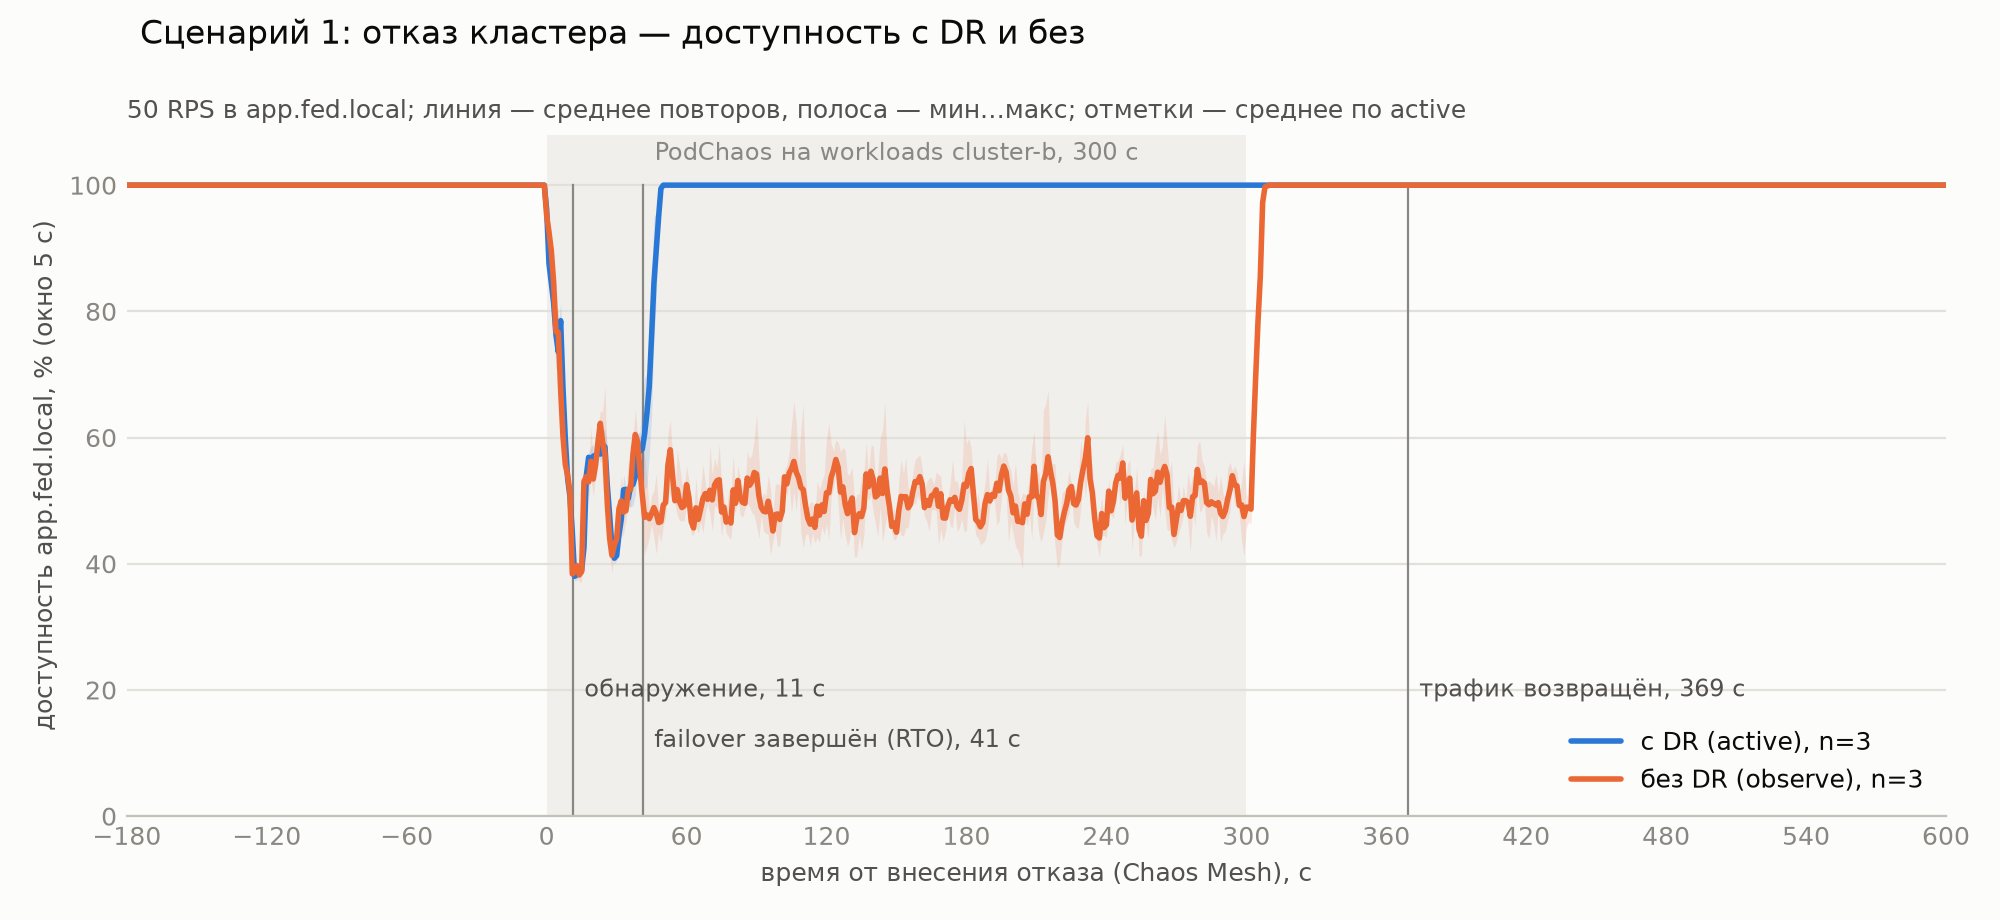
\includegraphics[width=\textwidth]{scenario1/task8-s1-availability.png}
  \caption{Доступность долгоживущего сервиса при отказе кластера с
  контроллером восстановления и без него (среднее трёх повторов)}
  \label{fig:s1}
\end{figure}

Снижение потерь по парам прогонов составило 86.8\%, 87.1\% и 87.3\%.
Оставшиеся потери приходятся на интервал от внесения отказа до переключения
трафика (около 41~с при половине трафика, направленной на отказавший
кластер). RTO складывается из времени обнаружения и 30~с подтверждения
отказа; эта задержка является платой за защиту от ложного переключения.

\section{Сценарий 2: деградация сети}

При разрабатываемом планировщике доля ошибок в окне отказа составила 2.40\%
против 4.41\% при наивном, то есть на 45.6\% меньше при цели не менее 20\%.
Разрабатываемый планировщик лучше наивного в каждой из трёх пар прогонов:
снижение составило 39.2\%, 50.5\% и 47.1\% (рис.~\ref{fig:s2}).

\begin{figure}[ht]
  \centering
  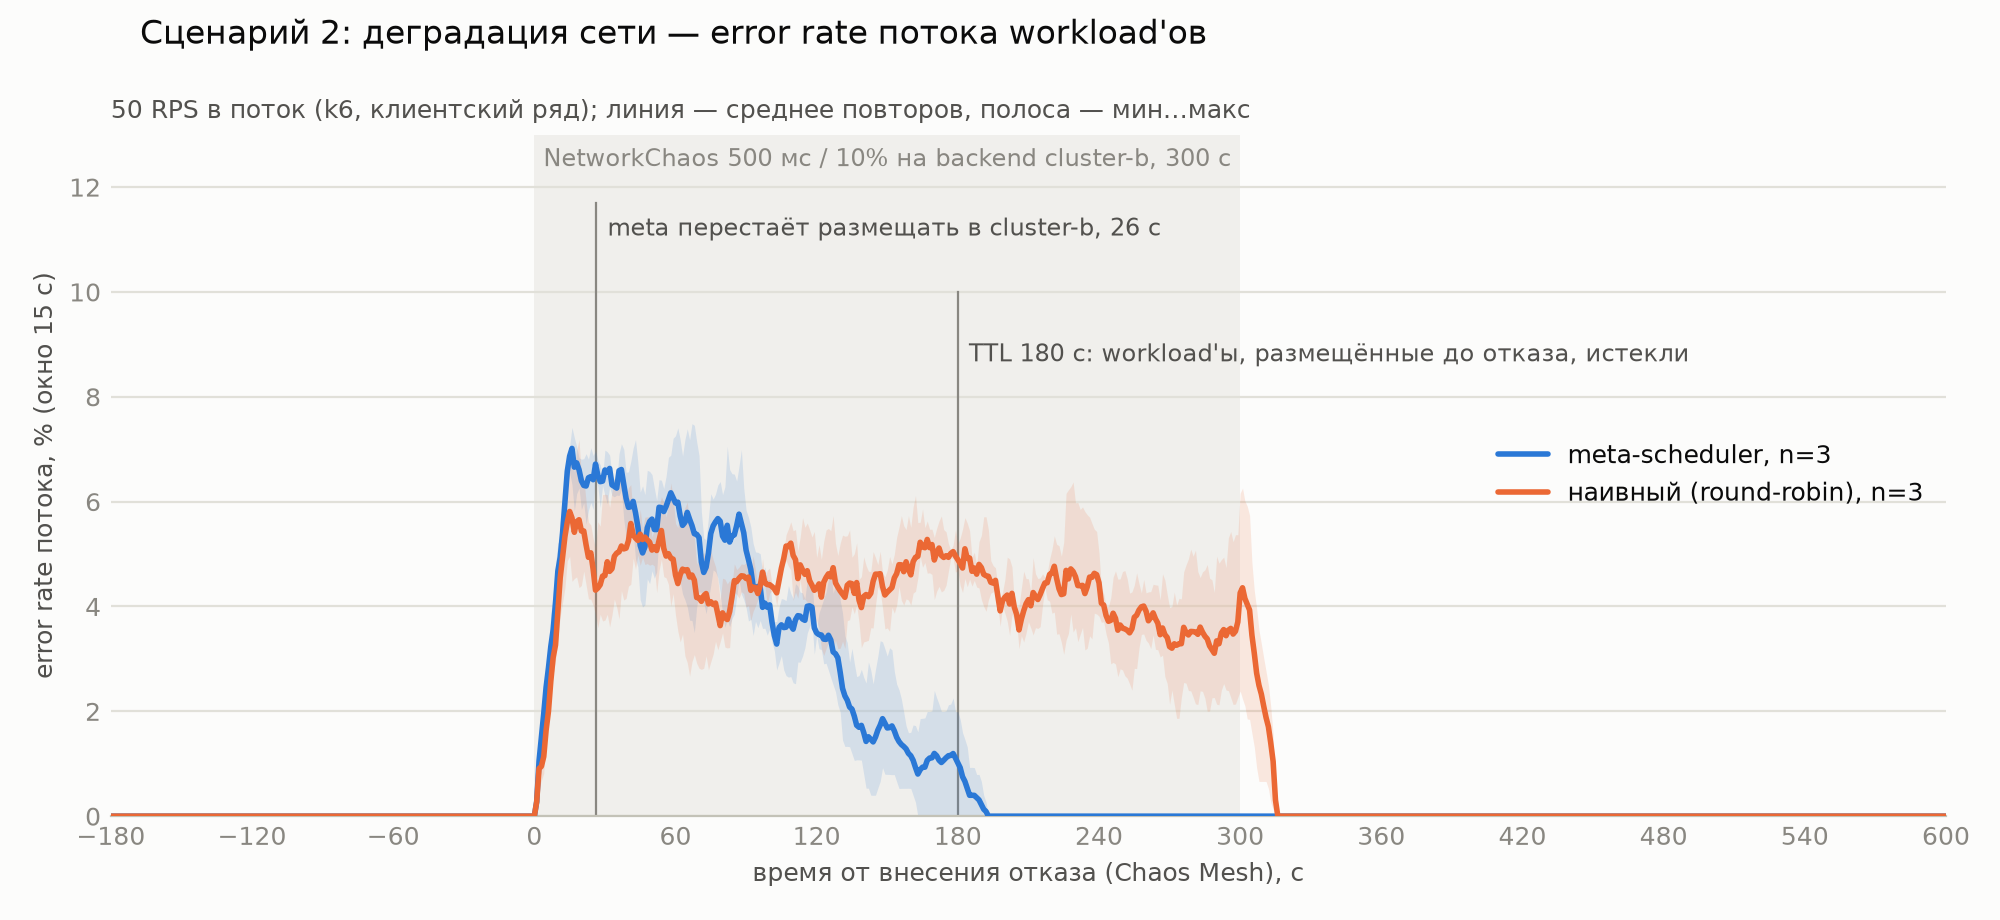
\includegraphics[width=\textwidth]{scenario2/task8-s2c-error-rate.png}
  \caption{Доля ошибок потока нагрузок при деградации сети в кластере B:
  разрабатываемый и наивный планировщики (среднее трёх повторов)}
  \label{fig:s2}
\end{figure}

Механизм эффекта виден по журналу решений: за время отказа разрабатываемый
планировщик не отправил в деградировавший кластер ни одного из 30
размещений, наивный~--- 15 из 29. Снижение оценки кластера в каталоге
наступает через 20--24~с после внесения отказа, первое решение в обход
деградировавшего кластера~--- через 25--27~с. Остаточные ошибки
разрабатываемого планировщика порождают нагрузки, размещённые в кластере B до
отказа: планировщик влияет только на новые размещения и не переносит уже
размещённые. Поэтому в первые 180~с отказа, пока эти нагрузки не завершились,
снижение составляет лишь 15.3\% (4.00\% против 4.72\%), а затем ошибки
разрабатываемого планировщика практически исчезают. Серверный ряд совпадает
с клиентским с точностью до 0.1 процентного пункта.

Кроме того, у наивного планировщика 5 из 87 размещений не перешли в
готовое состояние, у разрабатываемого~--- 0 из 87. Этот вред доля ошибок не
отражает, поскольку на неготовую нагрузку трафик не направляется.

\section{Сценарий 3: нарушение политики}

В режиме контроля не размещён ни один из 15 нарушителей, и каждая попытка
записана в журнал с корректным перечнем допустимых кластеров
(табл.~\ref{tab:s3}).

\begin{table}[ht]
  \centering
  \caption{Сценарий 3: три прогона по пять попыток}
  \label{tab:s3}
  \small
  \begin{tabularx}{\textwidth}{@{}>{\raggedright\arraybackslash}Xcccc@{}}
    \toprule
    Режим политик & Отклонено & Размещено & В журнале & \makecell{Задержка фиксации,\\медиана / макс.} \\
    \midrule
    Контроль & 15 из 15 & 0 & 15 & 4.7 / 9.9 с \\
    Аудит & 0 из 15 & 15 & 15 & 3.3 / 9.4 с \\
    Аудит, фиксация через отчёты политик & 0 из 15 & 15 & 15 & 3.3 / 30.2 с \\
    \bottomrule
  \end{tabularx}
\end{table}

Задержка фиксации нарушения ограничена периодом опроса (10~с). Фиксация через
отчёты политик медленнее: отчёт появляется в среднем через 23~с после
события Kyverno.

\section{Чувствительность к весам оценки}

Решения планировщика пересчитаны офлайн по записанным снимкам метрик для 66
точек симплекса весов с шагом 0.1 (181 решение, из них 59 в окне отказа).
Пересчёт совпадает с оценками планировщика с точностью $10^{-9}$. При
базовых весах доля размещений в деградировавший кластер равна 0\%, у
наивного планировщика~--- 51.7\%. Разрабатываемый планировщик лучше
наивного в 64 из 65 точек с $w_1 + w_2 > 0$ (рис.~\ref{fig:sensitivity}).
Единственное исключение~--- веса $(0.1, 0.0, 0.9)$: почти весь вес
приходится на загрузку, задержка не учитывается, и доля размещений в
деградировавший кластер составляет 59.3\%.

\begin{figure}[ht]
  \centering
  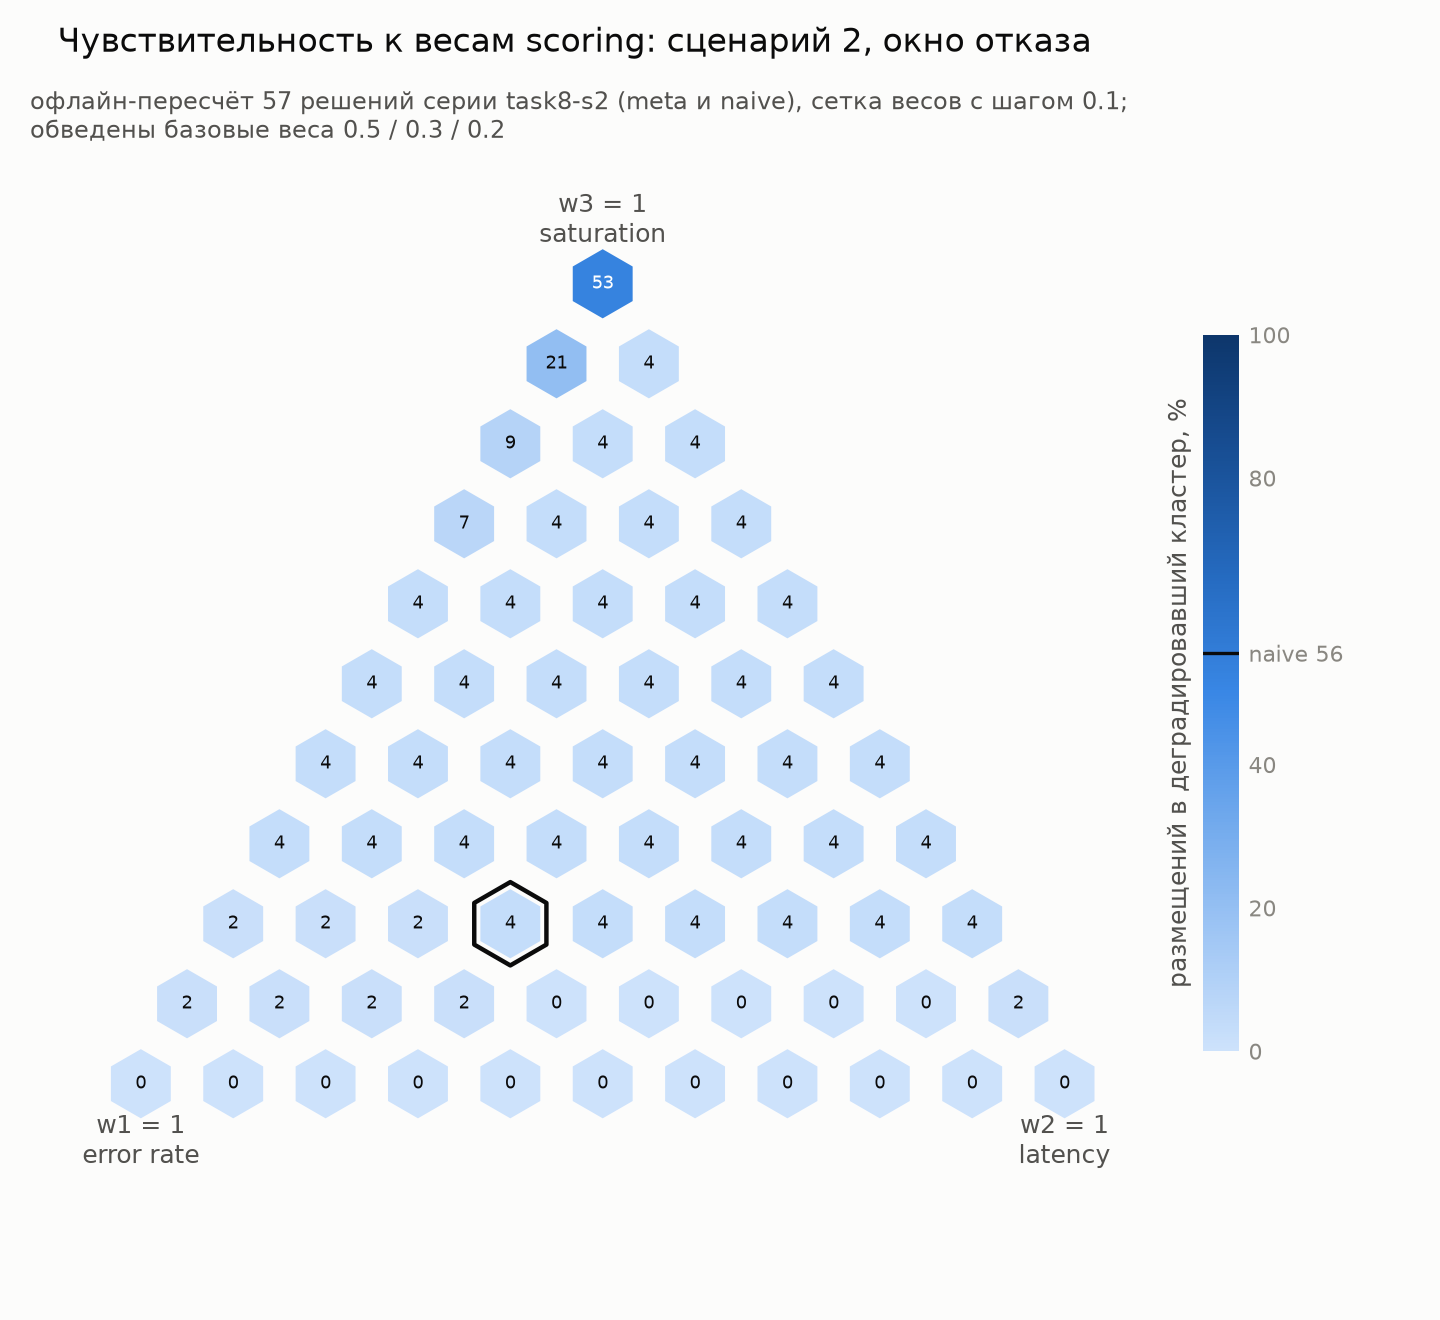
\includegraphics[width=0.75\textwidth]{task9/sensitivity.png}
  \caption{Доля размещений в деградировавший кластер в зависимости от весов
  оценки; обведены базовые веса}
  \label{fig:sensitivity}
\end{figure}

\section{Сравнение с другими методами выбора кластера}

\todo{Сравнение с другими методами выбора кластера: случайный выбор, выбор
по наименьшей загрузке, пороговый фильтр деградировавших кластеров~---
офлайн-пересчёт по записанным снимкам метрик (доля размещений в
деградировавший кластер). Раздел будет написан после проведения анализа.}

\section{Трассировка}

При доле записываемых трейсов 10\% собраны полные трейсы для 903--907 из
9000 запросов прогона. В штатном режиме серверная часть запроса занимает
около 0.5~мс по медиане: шлюз~--- 0.1~мс, переход из управляющего кластера в
кластер федерации~--- 0.2~мс, frontend~--- 0.04~мс, сеть до backend~---
0.14~мс. Накладные расходы трассировки неразличимы на фоне шума стенда:
медиана клиентской задержки составляет 0.83--1.03~мс при доле
записываемых трейсов 0\%, 10\% и 100\%, тогда как p95 между повторами одного
режима меняется от 2.3 до 6~мс.

\section{Достоверность данных каталога}

Снимки метрик, по которым принимал решения планировщик, сверены с рядами
Prometheus (732 снимка): доля ошибок совпадает в пределах 1 процентного
пункта в 98.1\% случаев, задержка p95 в пределах 10\%~--- в 99.6\% случаев.
Расхождения приходятся на моменты внесения и снятия отказа, когда ряд
изменяется на единицы процентных пунктов за 10~с: каталог получает данные в
реальном времени, а выгрузка выполняется позже по полным данным.

\chapter{Обсуждение результатов}
\label{ch:discussion}

Помимо достижения целевых показателей, в работе получены три результата,
касающиеся самого измерения: определена область, в которой преимущество
планировщика исчезает; показано, что серверный показатель доступности
федерации не видит отказа кластера; обнаружено, что механизмы
самовосстановления Kubernetes могут усиливать сетевой отказ.

\section{Отрицательный результат: устойчивость к весам}

Гипотеза H5 была сформулирована строго~--- «во всех точках сетки»~--- и не
подтвердилась в одной точке из 65. В этой точке 0.9 веса приходится на
загрузку, а задержка не учитывается. Причина понятна: на стенде все узлы
работают на одной физической машине, загрузка почти не зависит от
распределения нагрузки и не несёт информации о сетевой деградации. Вдоль
всей границы $w_2 = 0$ доля размещений в деградировавший кластер растёт по
мере уменьшения веса доли ошибок, поскольку доля ошибок при сетевой
деградации нарастает медленно. Отсюда следует, что метод работает, пока
в оценке присутствует метрика, чувствительная к типу отказа: для сетевой
деградации это задержка. Заранее зафиксированные веса $(0.5, 0.3, 0.2)$
находятся далеко от проблемной области.

\section{Серверный показатель доступности не видит отказа кластера}

Первоначально глобальная доступность федерации вычислялась как сумма
серверных метрик frontend всех кластеров. При отказе кластера целиком его
запросы завершаются ошибкой на шлюзе и до frontend не доходят, то есть
выпадают из знаменателя. В прогонах без переключения трафика клиент
наблюдал 49.9\% ошибок, шлюз~--- 47.5\%, а серверный показатель всё это
время показывал 0\% ошибок.

Это прямой ответ на вопрос об измерении надёжности мультикластерного
сервиса: агрегация серверных показателей кластеров слепа к отказу
кластера, и доступность федерации необходимо измерять в точке входа
трафика. Показатель перенесён на шлюз, серверный ряд оставлен для
диагностики. Проверка на выгруженных рядах шлюза показала, что скорость
расходования бюджета ошибок за 5~минут при отказе достигает 49, то есть
бюджет ошибок расходуется в 49 раз быстрее допустимого для цели 99\%.

\section{Самовосстановление усиливает сетевой отказ}

В первой серии экспериментов сценария~2 проверки работоспособности backend
выполнялись с таймаутом 1~с. При задержке 500~мс и потере 10\% пакетов
kubelet принимал медленный, но работающий backend за неработающий и
перезапускал его. В результате backend был недоступен от 24\% до 83\%
времени отказа и восстанавливался до 159~с после снятия отказа: сетевая
деградация превращалась в отказ сервиса.

Проверки были исправлены с учётом допустимой задержки сети, и серия
повторена; приёмка гипотез выполнена по повторной серии. Первая серия
сохранена как самостоятельный результат: в ней доля ошибок у наивного
планировщика втрое выше (16.34\% против 4.41\%), а снижение у
разрабатываемого~--- больше (64.4\%). Практический вывод: таймауты проверок
работоспособности должны учитывать допустимую задержку сети, иначе
самовосстановление само становится источником отказа.

\section{Почему не сработал алерт по бюджету ошибок}

Несрабатывание алерта является свойством многооконных правил~\cite{sre-workbook},
а не дефектом. Быстрый алерт требует более 14.4\% ошибок за час, то есть при
50 запросах в секунду около 23~тысяч ошибок. Наиболее тяжёлый инцидент на
стенде (отказ без переключения трафика) дал до 7025 ошибок и 0.60\% месячного
бюджета. Для коротких инцидентов быстрее срабатывает не алерт по бюджету
ошибок, а собственный мониторинг контроллера восстановления (TTD 11~с).

\section{Ограничения и угрозы достоверности}

\begin{itemize}
  \item \textbf{Одна машина.} Абсолютные значения (задержки, TTD) зависят от
        стенда и на реальные системы не переносятся. Сравнения выполнены в
        одинаковых условиях и переносятся как направление эффекта.
  \item \textbf{Два кластера федерации.} После деградации одного из них у
        планировщика остаётся единственный кандидат, а результат получен
        для одного значения числа кластеров.
  \item \textbf{Три повтора без статистического теста.} Это компенсируется
        требованием одинакового знака эффекта в каждой паре: снижение доли
        ошибок по парам составило от 39\% до 51\%, потерь запросов~--- от
        86.8\% до 87.3\%.
  \item \textbf{Малоинформативная загрузка.} Узлы делят одну машину, и вклад
        третьего слагаемого оценки мал.
  \item \textbf{Нейтральная оценка кластера без трафика.} Кластер без
        метрик получает оценку около 0.55 против около 0.95 у кластера с
        трафиком, поэтому с холодного старта планировщик собирает поток в
        одном кластере. На стенде это обойдено фоновой нагрузкой; в формуле
        это ограничение сохраняется.
  \item \textbf{Только новые размещения.} Планировщик не переносит уже
        размещённые нагрузки, поэтому его эффект ограничен скоростью
        обновления потока.
  \item \textbf{Единая точка отказа прототипа.} Управляющий кластер и шлюз
        не дублируются; в реальной системе их резервирование обязательно,
        но в задачу работы оно не входило.
  \item \textbf{Нагрузка без состояния.} Репликация данных и допустимая
        потеря данных не рассматривались.
\end{itemize}

\unnumchapter{Выводы}

По каждой из поставленных задач получены следующие результаты.

\begin{enumerate}
  \item Проведён обзор средств управления федерацией, наблюдаемости,
        аварийного восстановления и контроля политик. Установлено, что
        существующие федеративные планировщики выбирают кластер по
        статическим атрибутам, а ни одно из рассмотренных решений не
        объединяет политики, текущие показатели качества и состояние
        кластеров в одно решение о размещении.
  \item Развёрнут экспериментальный стенд из управляющего кластера и двух
        кластеров федерации с тестовым сервисом, шлюзом и генератором
        нагрузки. Стенд и каждый эксперимент воспроизводятся из
        репозитория одной командой.
  \item Построен слой наблюдаемости федерации: метрики кластеров
        агрегируются через Thanos, определены локальные и глобальные
        показатели уровня обслуживания, реализована сквозная трассировка с
        разложением задержки по звеньям. Показано, что доступность
        федерации необходимо измерять в точке входа трафика: сумма
        серверных показателей кластеров не видит отказа кластера.
  \item Разработан каталог кластеров, хранящий атрибуты кластеров, их
        текущее состояние, журнал решений о размещении со всеми
        кандидатами, журнал нарушений политик и инцидентов. Метрики
        каталога совпадают с исходными рядами в 98--99\% снимков.
  \item Реализованы двухуровневые политики размещения. В режиме контроля
        не размещён ни один из 15 нарушителей, все попытки зафиксированы в
        журнале в течение не более 10~с.
  \item Разработан планировщик уровня федерации, оценивающий кластеры по
        текущим доле ошибок, задержке и загрузке, и наивный планировщик,
        выбирающий кластеры по очереди среди тех же допустимых кандидатов.
  \item Разработан контроллер аварийного восстановления на основе конечного
        автомата с асимметричными переходами. Время обнаружения отказа
        составило 10.6--12.8~с, время восстановления~--- 40.7--42.9~с при
        целевых значениях 60~с и 5~мин.
  \item Проведены эксперименты по трём сценариям отказов. Контроллер
        восстановления снижает число потерянных запросов при отказе
        кластера на 87.1\%. Разрабатываемый планировщик снижает долю ошибок
        при деградации сети на 45.6\% относительно наивного, превосходя его
        в каждой паре прогонов.
  \item Проведён анализ результатов. Преимущество планировщика сохраняется
        в 64 из 65 комбинаций весов и исчезает, когда оценка не учитывает
        задержку. Обнаружено, что проверки работоспособности с таймаутом,
        не учитывающим задержку сети, превращают сетевую деградацию в отказ
        сервиса.
\end{enumerate}

\unnumchapter{Заключение}

\todo{Заключение~--- черновик, требует ручной доработки.}

В работе разработана система управления размещением нагрузки в федерации
Kubernetes-кластеров с учётом метрик надёжности. Система построена как
сквозной контур управления, связывающий наблюдаемость, показатели уровня
обслуживания, политики размещения, выбор кластера и аварийное
восстановление, и экспериментально оценена на воспроизводимых отказах. Все
целевые показатели достигнуты, а в центральном сценарии планировщик,
учитывающий текущие метрики кластеров, даёт на 45.6\% меньше ошибок, чем
наивный выбор.

Получены ответы на поставленные исследовательские вопросы.

Локальные показатели кластеров корректно агрегируются через Thanos и служат
входными данными планировщика. Однако глобальную доступность федерации так
вычислять нельзя: сумма серверных показателей не видит отказа кластера, и
доступность необходимо измерять в точке входа трафика.

Оба исследованных механизма дают измеримый эффект: переключение трафика
снижает потери запросов при отказе кластера на 87.1\%, а размещение с учётом
метрик снижает долю ошибок при деградации сети на 45.6\%. Встроенное
самовосстановление Kubernetes с проверками по умолчанию, напротив, усиливает
сетевой отказ.

Цикл аварийного восстановления выполняется программно и воспроизводим: время
обнаружения отказа не превышает 13~с, время восстановления~--- 43~с во всех
прогонах. Времена отсчитываются от событий инструмента внесения отказа, а
фазы инцидента записываются в каталог.

Политики размещения выражены требованиями нагрузки и описанием кластера и
исполняются на двух независимых рубежах; ни один нарушитель не был размещён.

Планировщик, использующий метрики из каталога, превосходит выбор по очереди
при тех же обязательных ограничениях в каждой паре прогонов. Его
преимущество устойчиво к выбору весов, пока оценка учитывает метрику,
чувствительную к типу отказа.

Направления дальнейшей работы: исследование зависимости эффекта
планировщика и накладных расходов контура от числа кластеров; перенос уже
размещённых нагрузок при деградации кластера; иная оценка кластеров без
трафика вместо нейтральных значений; оценка доверительных интервалов при
большем числе повторов; резервирование управляющего контура и шлюза.

% Источники в порядке первого упоминания в тексте.
% Оформление близко к ГОСТ Р 7.0.100--2018; адреса и даты обращения
% проверить перед сдачей.
\begin{thebibliography}{99}
\addcontentsline{toc}{chapter}{Список литературы}

\bibitem{k8s} Kubernetes Documentation [Электронный ресурс]. --- URL:
  \url{https://kubernetes.io/docs/} (дата обращения: 06.11.2026).

\bibitem{kubefed} Kubernetes Cluster Federation (KubeFed) [Электронный
  ресурс]. --- URL: \url{https://github.com/kubernetes-retired/kubefed}
  (дата обращения: 06.11.2026).

\bibitem{admiralty} Admiralty Documentation [Электронный ресурс]. --- URL:
  \url{https://admiralty.io/docs/} (дата обращения: 06.11.2026).

\bibitem{liqo} Liqo Documentation [Электронный ресурс]. --- URL:
  \url{https://docs.liqo.io/} (дата обращения: 06.11.2026).

\bibitem{ocm} Open Cluster Management: Placement [Электронный ресурс]. ---
  URL: \url{https://open-cluster-management.io/docs/concepts/content-placement/placement/}
  (дата обращения: 06.11.2026).

\bibitem{karmada} Karmada Documentation [Электронный ресурс]. --- URL:
  \url{https://karmada.io/docs/} (дата обращения: 06.11.2026).

\bibitem{prometheus} Prometheus Documentation [Электронный ресурс]. ---
  URL: \url{https://prometheus.io/docs/} (дата обращения: 06.11.2026).

\bibitem{thanos} Thanos Documentation [Электронный ресурс]. --- URL:
  \url{https://thanos.io/tip/thanos/getting-started.md/} (дата обращения:
  06.11.2026).

\bibitem{cortex} Cortex Documentation [Электронный ресурс]. --- URL:
  \url{https://cortexmetrics.io/docs/} (дата обращения: 06.11.2026).

\bibitem{mimir} Grafana Mimir Documentation [Электронный ресурс]. --- URL:
  \url{https://grafana.com/docs/mimir/latest/} (дата обращения: 06.11.2026).

\bibitem{victoriametrics} VictoriaMetrics Documentation [Электронный
  ресурс]. --- URL: \url{https://docs.victoriametrics.com/} (дата обращения:
  06.11.2026).

\bibitem{sre-book} Site Reliability Engineering: How Google Runs Production
  Systems / B.~Beyer, C.~Jones, J.~Petoff, N.~R.~Murphy (eds.). ---
  Sebastopol: O'Reilly Media, 2016. --- 552~p.

\bibitem{sre-workbook} The Site Reliability Workbook: Practical Ways to
  Implement SRE / B.~Beyer, N.~R.~Murphy, D.~K.~Rensin, K.~Kawahara,
  S.~Thorne (eds.). --- Sebastopol: O'Reilly Media, 2018. --- 508~p.

\bibitem{pyrra} Pyrra: SLOs with Prometheus [Электронный ресурс]. --- URL:
  \url{https://github.com/pyrra-dev/pyrra} (дата обращения: 06.11.2026).

\bibitem{sloth} Sloth: Prometheus SLO generator [Электронный ресурс]. ---
  URL: \url{https://sloth.dev/} (дата обращения: 06.11.2026).

\bibitem{otel} OpenTelemetry Documentation [Электронный ресурс]. --- URL:
  \url{https://opentelemetry.io/docs/} (дата обращения: 06.11.2026).

\bibitem{velero} Velero Documentation [Электронный ресурс]. --- URL:
  \url{https://velero.io/docs/} (дата обращения: 06.11.2026).

\bibitem{argo-rollouts} Argo Rollouts Documentation [Электронный ресурс]. ---
  URL: \url{https://argo-rollouts.readthedocs.io/} (дата обращения:
  06.11.2026).

\bibitem{flagger} Flagger Documentation [Электронный ресурс]. --- URL:
  \url{https://docs.flagger.app/} (дата обращения: 06.11.2026).

\bibitem{chaos-mesh} Chaos Mesh Documentation [Электронный ресурс]. ---
  URL: \url{https://chaos-mesh.org/docs/} (дата обращения: 06.11.2026).

\bibitem{litmus} LitmusChaos Documentation [Электронный ресурс]. --- URL:
  \url{https://docs.litmuschaos.io/} (дата обращения: 06.11.2026).

\bibitem{kyverno} Kyverno Documentation [Электронный ресурс]. --- URL:
  \url{https://kyverno.io/docs/} (дата обращения: 06.11.2026).

\bibitem{gatekeeper} OPA Gatekeeper Documentation [Электронный ресурс]. ---
  URL: \url{https://open-policy-agent.github.io/gatekeeper/website/docs/}
  (дата обращения: 06.11.2026).

\bibitem{kind} kind: Kubernetes in Docker [Электронный ресурс]. --- URL:
  \url{https://kind.sigs.k8s.io/} (дата обращения: 06.11.2026).

\bibitem{envoy-gateway} Envoy Gateway Documentation [Электронный ресурс]. ---
  URL: \url{https://gateway.envoyproxy.io/docs/} (дата обращения: 06.11.2026).

\bibitem{gateway-api} Kubernetes Gateway API [Электронный ресурс]. --- URL:
  \url{https://gateway-api.sigs.k8s.io/} (дата обращения: 06.11.2026).

\bibitem{jaeger} Jaeger Documentation [Электронный ресурс]. --- URL:
  \url{https://www.jaegertracing.io/docs/} (дата обращения: 06.11.2026).

\bibitem{trace-context} Trace Context: W3C Recommendation [Электронный
  ресурс]. --- URL: \url{https://www.w3.org/TR/trace-context/} (дата
  обращения: 06.11.2026).

\bibitem{fastapi} FastAPI Documentation [Электронный ресурс]. --- URL:
  \url{https://fastapi.tiangolo.com/} (дата обращения: 06.11.2026).

\bibitem{postgresql} PostgreSQL Documentation [Электронный ресурс]. --- URL:
  \url{https://www.postgresql.org/docs/} (дата обращения: 06.11.2026).

\bibitem{controller-runtime} controller-runtime [Электронный ресурс]. ---
  URL: \url{https://github.com/kubernetes-sigs/controller-runtime} (дата
  обращения: 06.11.2026).

\bibitem{k6} Grafana k6 Documentation [Электронный ресурс]. --- URL:
  \url{https://grafana.com/docs/k6/latest/} (дата обращения: 06.11.2026).

\end{thebibliography}

\appendix
\renewcommand{\thechapter}{\Asbuk{chapter}}
\titleformat{\chapter}[block]{\normalfont\large\bfseries\centering}{Приложение \thechapter.}{0.5em}{}
\addtocontents{toc}{\protect\renewcommand{\protect\cftchappresnum}{Приложение }}
\addtocontents{toc}{\protect\setlength{\protect\cftchapnumwidth}{8em}}

\chapter{Воспроизведение экспериментов}

Исходный код, конфигурация стенда, сценарии экспериментов и сырые данные
всех прогонов находятся в репозитории \url{https://github.com/hanglider/cursach}.
Требования к машине: docker с виртуальной машиной на 10~ГБ памяти.

\begin{table}[ht]
  \centering
  \caption{Основные действия}
  \small
  \begin{tabular}{@{}lll@{}}
    \toprule
    Действие & Команда & Время \\
    \midrule
    Развернуть стенд & \texttt{make stand-up} & около 3 мин \\
    Серия сценария 1 & \texttt{make dr-series} & около 1.5 ч \\
    Серия сценария 2 & \texttt{make sched-series} & 1.5--2 ч \\
    Серия сценария 3 & \texttt{make policy-series} & около 35 мин \\
    Анализ и графики & \texttt{make analysis}, \texttt{make plots} & минуты \\
    \bottomrule
  \end{tabular}
\end{table}

\chapter{Структура репозитория}

\begin{table}[ht]
  \centering
  \caption{Каталоги репозитория}
  \small
  \begin{tabularx}{\textwidth}{@{}lX@{}}
    \toprule
    Каталог & Содержимое \\
    \midrule
    \texttt{stand/} & Развёртывание стенда: кластеры, наблюдаемость, шлюз,
      политики \\
    \texttt{test-service/} & Тестовый сервис, Go \\
    \texttt{registry/} & Каталог кластеров, Python, FastAPI, PostgreSQL \\
    \texttt{scheduler/} & Планировщик уровня федерации и наивный
      планировщик, Go \\
    \texttt{dr-controller/} & Контроллер аварийного восстановления, Go \\
    \texttt{experiments/} & Сценарии отказов и нагрузки, сырые результаты \\
    \texttt{analysis/} & Обработка результатов, графики, проверка гипотез \\
    \texttt{docs/} & Постановка задачи, архитектура, принятые решения \\
    \bottomrule
  \end{tabularx}
\end{table}


\end{document}
